\chapter{初始化}
系统初始化是整个外包检索协议的基石。在数据上传前，DO 必须对明文空间进行代数化映射，构建从高维文本与连续数值到离散有限域元素的映射字典。
该过程涵盖密码学参数生成、关键字词表初始化以及数值前缀空间初始化。
\section{密码学参数生成}
令 $\lambda$ 为系统的安全参数。DO 首先初始化底层密码学原语：

\begin{itemize}
\item \textbf{哈希与伪随机函数：} 选择 BLAKE2b 作为底层哈希算法，实例化伪随机函数 $F: \{0,1\}^\lambda \times \{0,1\}^* \to \{0,1\}^{256}$。随机均匀地抽取一个字符串作为主对称密钥 $mk \leftarrow \{0,1\}^\lambda$。
\item \textbf{累加器参数初始化：} 调用累加器的 $KeyGen(1^\lambda, U)$ 算法，其中 $U$ 为系统支持的最大集合基数。系统随机选取隐藏私钥 $s \leftarrow \mathbb{Z}_p^*$，并基于双线性群 $\mathbb{G}_1, \mathbb{G}_2$ 生成公钥参数元组 $pk$。私钥 $sk$ 由 DO 妥善保管，公钥 $pk$ 公开发布。
\end{itemize}
\section{词表初始化}
我们期望将关键字密文压缩到NonZeroU16有两个原因。一是AttDigest索引节点会存储加密后的关键字集，相比直接存储通常是128位经过PRF加密后的数据，使用某种方式将密文限制在NonZeroU16的集合元素更节省空间。
二是对象关键字集是否包含请求关键字时，我们需要依靠累加器给出计算结果和证明。由于输入是任意字符串集合，若仅简单采用字节阶段压缩，从数学上无法避免碰撞。并且从效率上考虑，若关键字总量很小，其映射结果稀疏，
还必须设置构建公私钥的必要参数全集大小为65535。由于用户知道关键字全集，我们考虑让用户离线构建一个<token,tokenid>的键值对表上传至区块链。

具体来说，用户在本地先将明文关键字做规范化处理，用密钥Blake2b计算一个稳定token，按token排序，将排序后的第i个关键字分配编号i+1,这样就会得到一个在固定全集上的伪随机编号。
在构建索引时我们可以将仅仅将关键字密文的ID存储于索引节点，而不存储明文或者其哈希值。

但这样有一个缺陷在于，该设计没有限制住关键字对应的ID大小，词表可以实现零冲突但理论上可以无限增长，超出累加器所能处理的范围。
\section{前缀表初始化}
通过前缀转换函数\cite{xu2019vchain}$\mathbb{TR}(\cdot)$，一个数值可以转换为一组二进制元素。例如，4的二进制表示为100，它的前缀集可以表示$\mathbb{TR}(4) =\left\{1\ast,10\ast,100\right\}$,
其中$\ast$表示通配符匹配操作符。我们通常取能表达整个数据集的位数作为前缀二叉树深度，对于单维范围$[\alpha,\beta]$,我们首先将$\alpha,\beta$表示为二进制格式，将其视为整个二进制空间集树的最小叶节点，所能精确覆盖整个范围$[\alpha,\beta]$的最小树节点集合就是
所找的前缀集合。例如，对于一维范围$[0,6]$，首先构建位长为3的二进制空间集树，如图\ref{fig:prefix-tree}先将$0$和$6$作为树的两个叶子节点，最后找到覆盖其整个范围$[0,6]$的树节点的最小集合$\{\ast,10\ast,100\}$。
\begin{figure}[h]
    \centering
    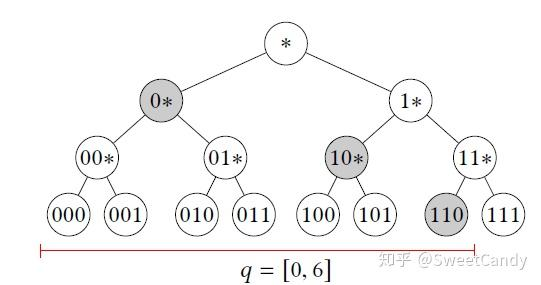
\includegraphics[width=0.5\textwidth]{figures/prefix-tree.png}
    \caption{二叉前缀树}
    \label{fig:prefix-tree}
\end{figure}
通过上述变换，查询一个数值$v$是否在区间$[\alpha,\beta]$内，就变成了将$v$的变换前缀集合与$[\alpha,\beta]$的等价集合进行布尔查询。在上述例子中，$4\in[0,6]$因为$\{1\ast,10\ast,100\}\cap\{0\ast,10\ast,110\} = \{10\ast\} \neq \emptyset$,
$7\notin[0,6]$因为$\{1\ast,11\ast,111\}\cap\{0\ast,10\ast,110\} = \emptyset$。

利用前缀转换，数值加密后的的范围查询实际上等同于在密文关键字查询，也就需要构造前缀集合的密文词表。用户已知表达整个数据集的所需位长，预先枚举所有前缀，每个前缀经过PRF得到token，token再映射到词表ID。

这样做有两个缺陷，一是前缀表大小是所表达数值个数的两倍。若数据表示位数4，则枚举前缀集合共有31个元素。我们限定集合元素大小为U16,那么数据最大位长为15，所能表示最大数据为32768。二是若用户给定的位数参数很小，则候选空间本身就很小，结合查询模式、访问模式、频率信息，服务端
很容易做枚举或统计推断。第二个问题没有在词表中出现是因为词表的输入空间是无限的，而数值的输入空间有限。不过这点待定，如果服务器不知道当前索引是范围索引呢？在它视图下仅仅是一个特殊的关键字索引？
\section{本章小结}
本章详细介绍了系统初始化阶段的关键步骤，包括密码学参数生成、密文词表初始化以及前缀表初始化。通过规范化、确定性令牌生成和保序扰乱等技术手段，系统成功将高维文本与连续数值映射为离散的有限域元素，为后续的加密索引构建和可验证查询处理奠定了坚实的基础。